\subsection{Task 2.1 -- Activity diagram}

\subsubsection{Luồng đặt và thanh toán}
Sơ đồ theo UC-01 từ giỏ hàng đến kết quả thanh toán. Swimlane phân biệt thao tác của khách, Next.js và NestJS. Khi mở checkout, giao diện tải trạng thái thanh toán và chi tiết đơn song song. Khi giỏ không hợp lệ, khách quay lại sửa giỏ. Đơn thẻ lỗi còn hạn có thể thử lại; đơn hết hạn chỉ trả kho khi đủ điều kiện hủy.

\begin{center}
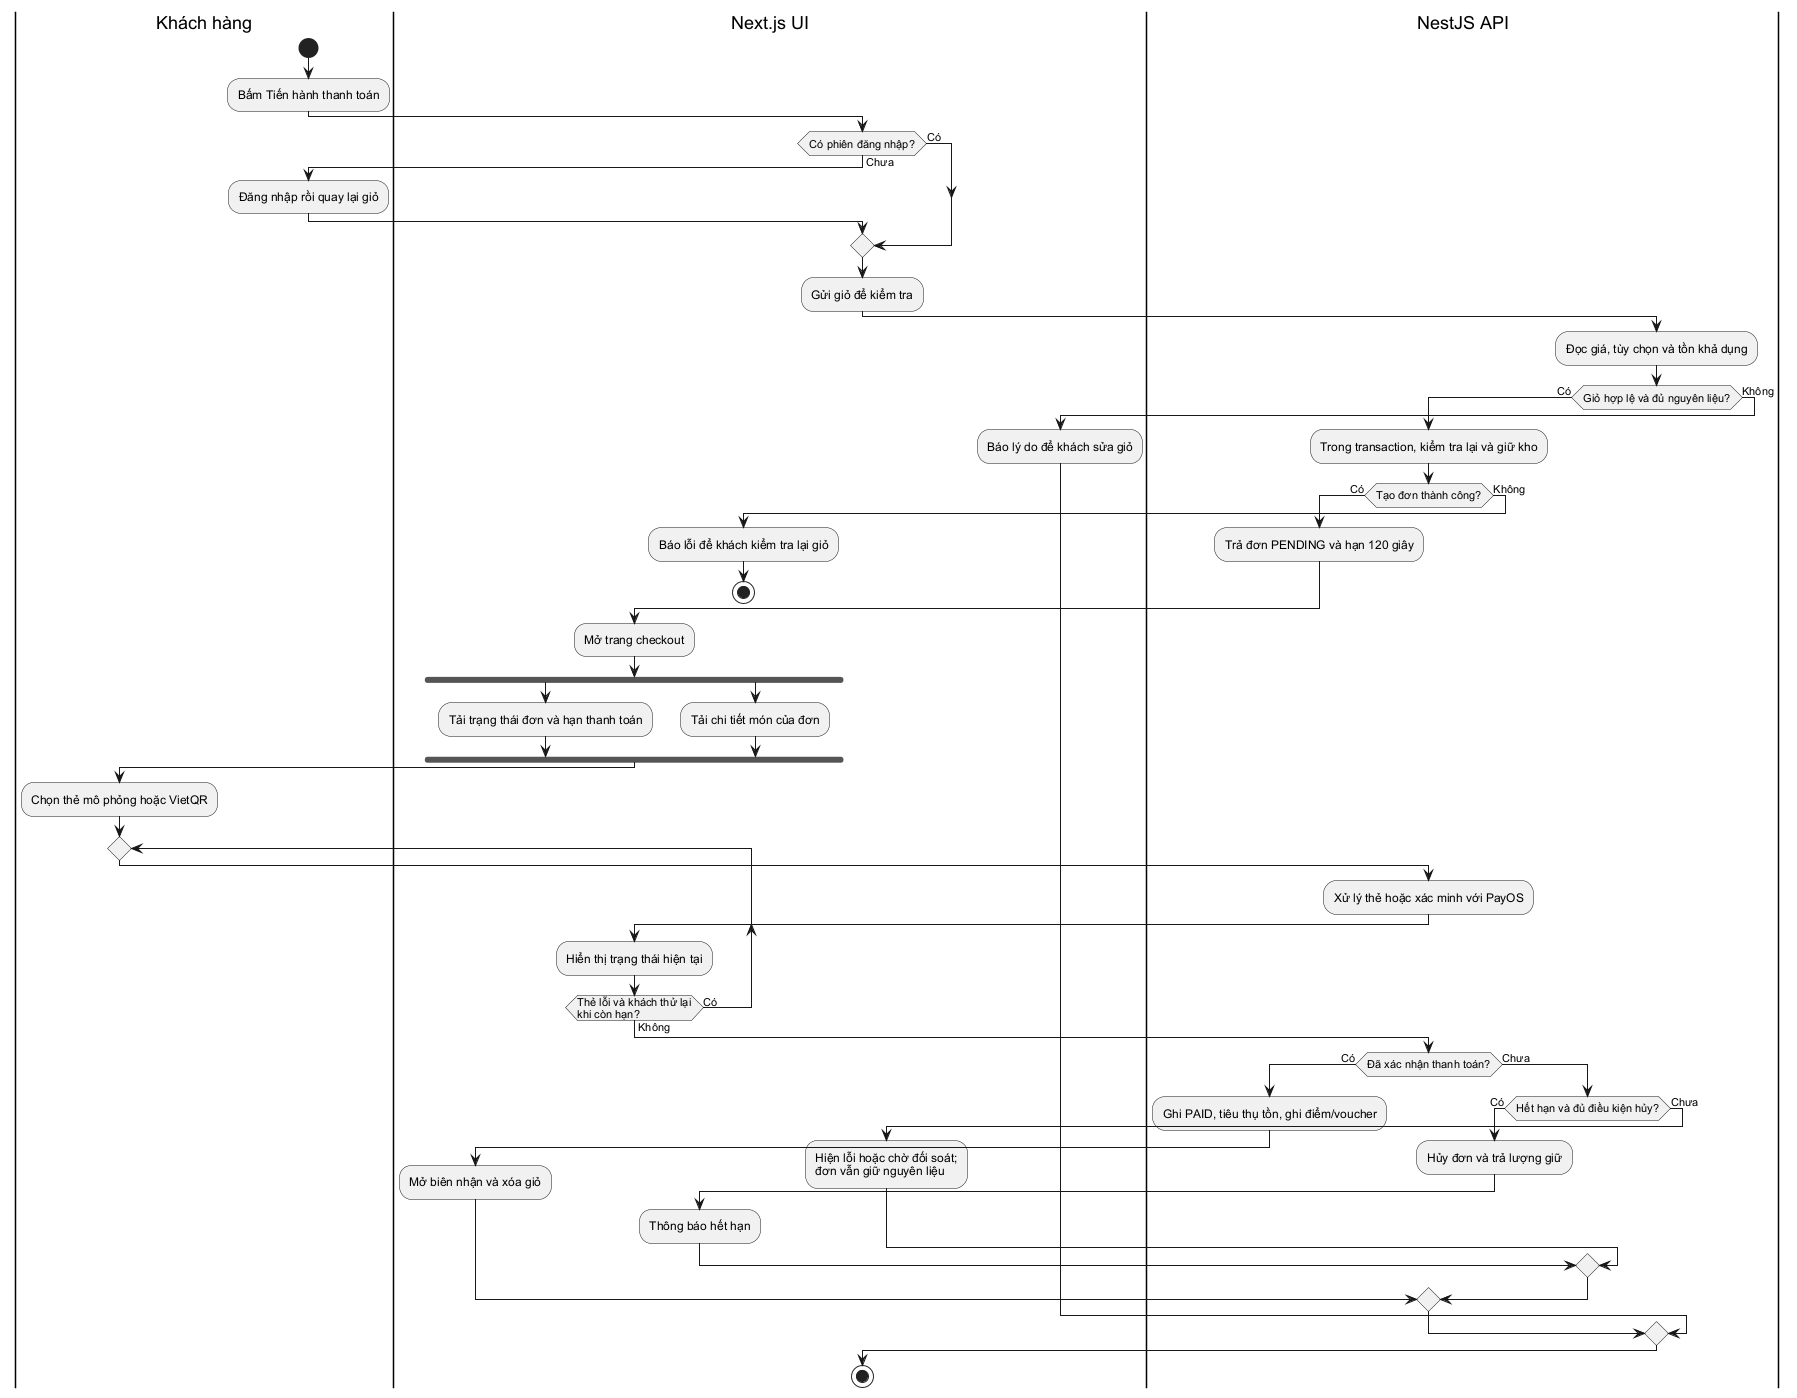
\includegraphics[width=\linewidth,height=0.70\textheight,keepaspectratio]{../../diagrams/activity-checkout-overview.png}\\[0.5em]
{\small\itshape Hình 2.1a. Hoạt động đặt và thanh toán đơn hàng}
\end{center}

\clearpage
\subsubsection{Kiểm tra giỏ và giữ nguyên liệu}
API kiểm tra giỏ ở chế độ chỉ đọc. Hai truy vấn món kèm giá và topping được khởi chạy cùng lúc. API chờ đủ hai kết quả trước khi đọc công thức. Khi tạo đơn, API tính giá và ưu đãi, sau đó kiểm tra lại giá và tăng lượng giữ bằng lệnh cập nhật có điều kiện đủ tồn trong transaction. Đơn, dòng món và lượng giữ được ghi cùng nhau. Khi thiếu nguyên liệu hoặc có lỗi ghi, transaction được hoàn tác.

\begin{center}
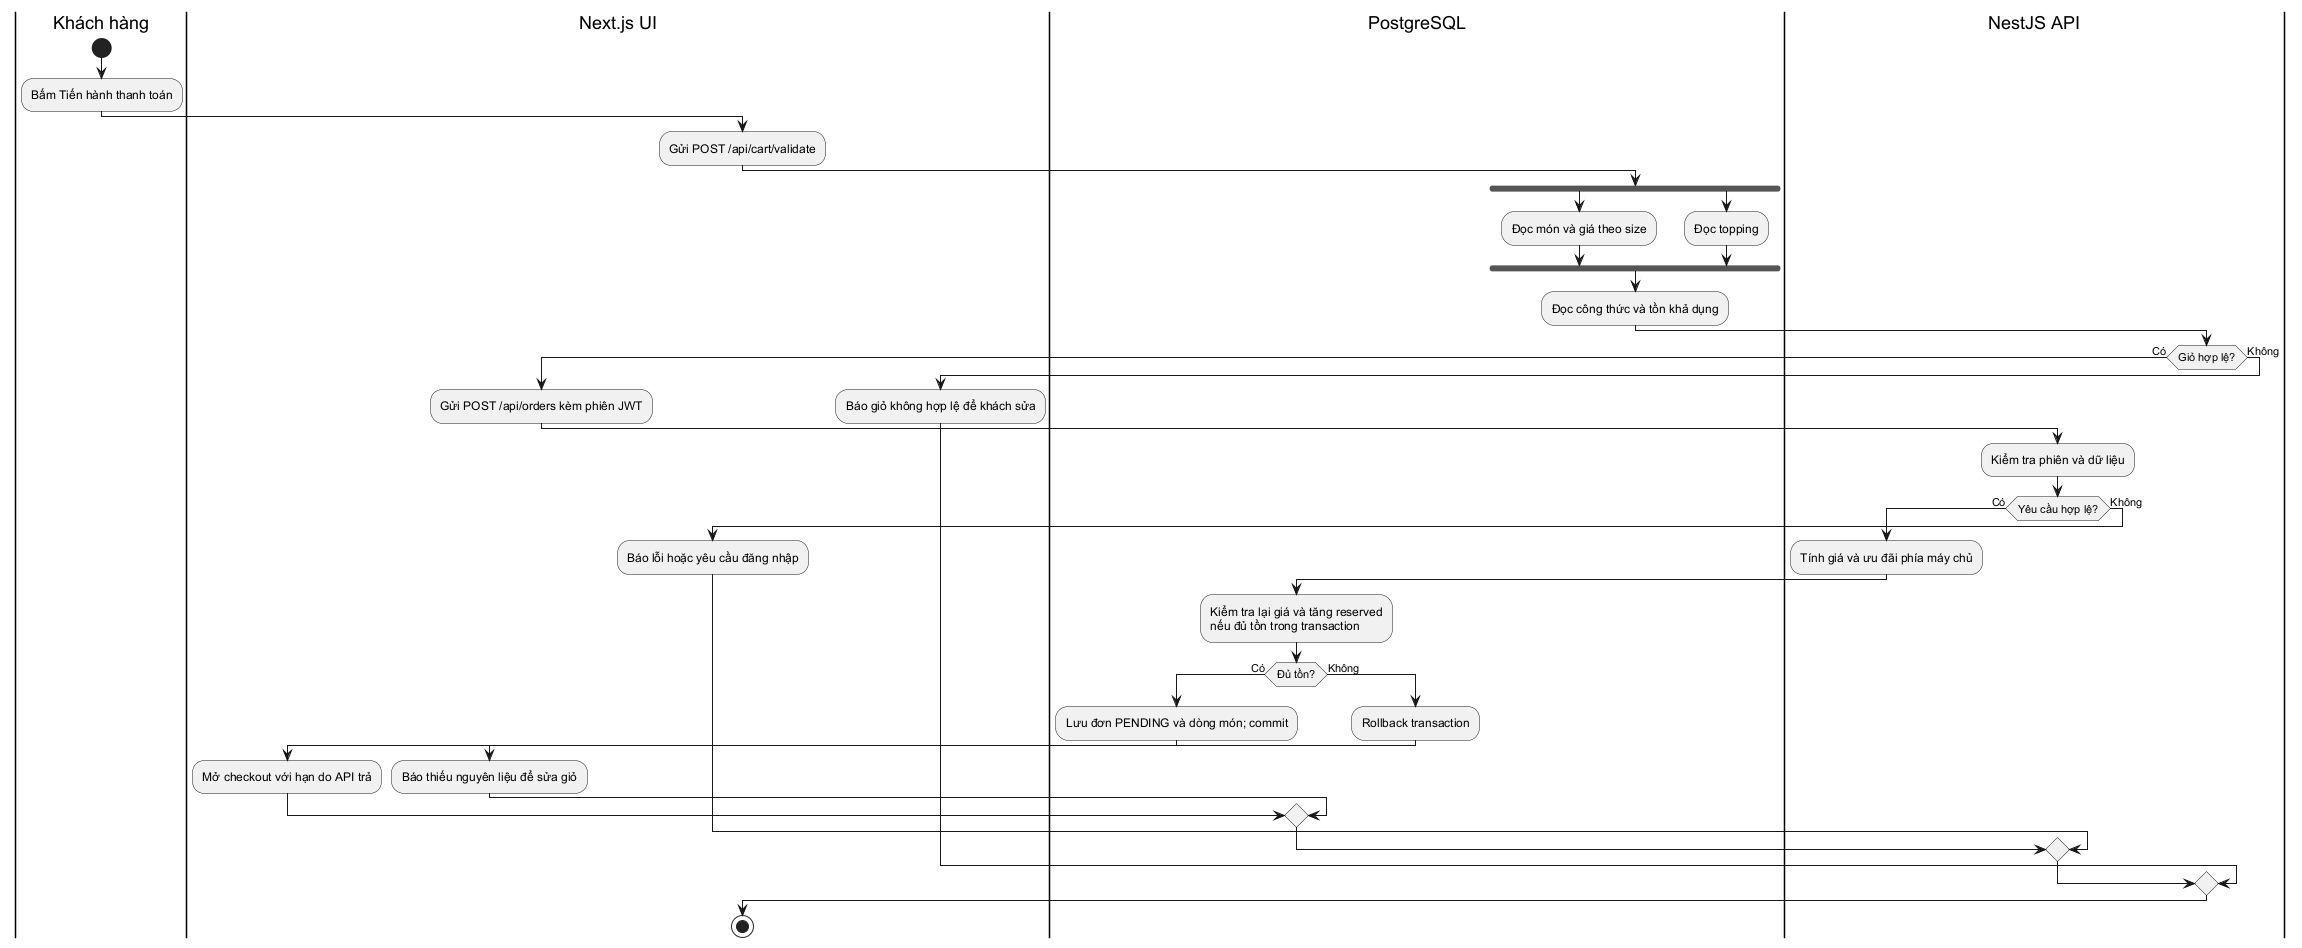
\includegraphics[width=\linewidth,height=0.70\textheight,keepaspectratio]{../../diagrams/activity-order-reservation.png}\\[0.5em]
{\small\itshape Hình 2.1b. Kiểm tra giỏ và giữ nguyên liệu}
\end{center}

\clearpage
\subsubsection{Thanh toán thẻ mô phỏng và chống xử lý lặp}
Khóa \texttt{Idempotency-Key} gắn với bản ghi \texttt{Payment}. Yêu cầu lặp trả kết quả đã ghi. Nếu thẻ thất bại, API ghi \texttt{FAILED}, đơn chuyển sang \texttt{PAYMENT\_FAILED} và giữ kho đến khi đơn được thanh toán hoặc đủ điều kiện hủy.

\begin{center}
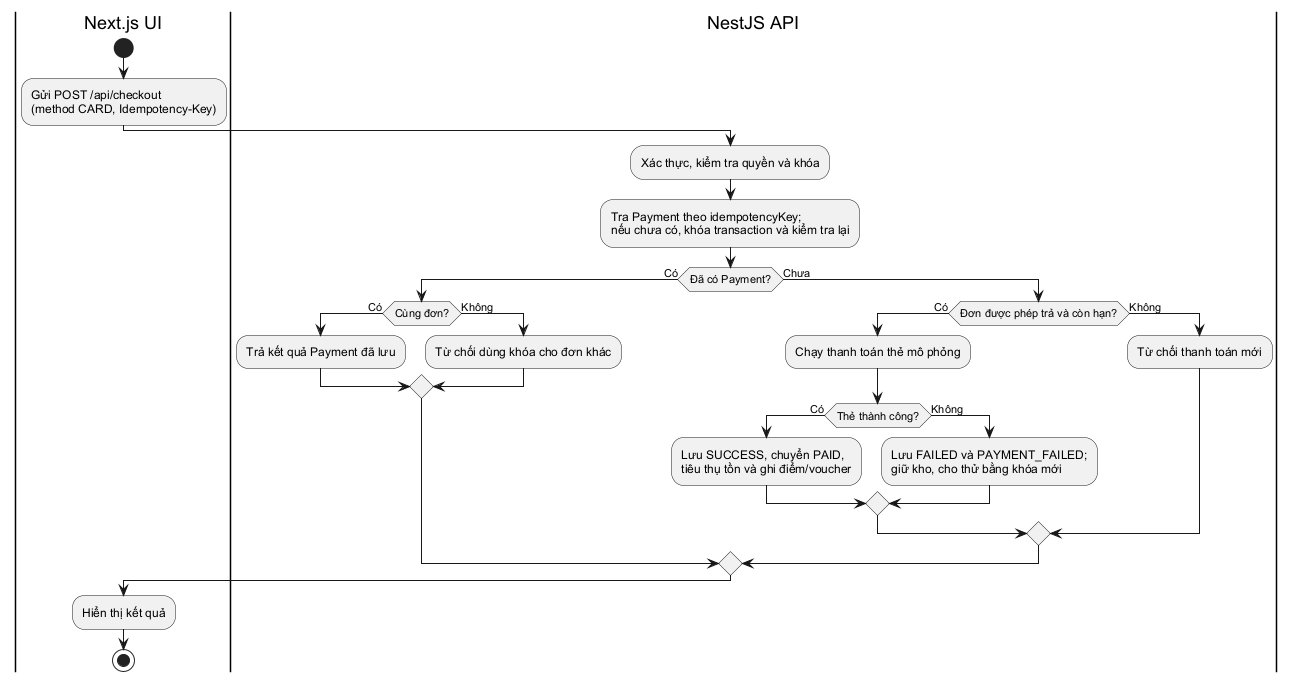
\includegraphics[width=\linewidth,height=0.70\textheight,keepaspectratio]{../../diagrams/activity-idempotency.png}\\[0.5em]
{\small\itshape Hình 2.1c. Xử lý thẻ mô phỏng}
\end{center}

\clearpage
\subsubsection{VietQR, webhook và đối soát}
Webhook có chữ ký hợp lệ hoặc kết quả đối soát trực tiếp có thể xác nhận đã nhận đủ tiền. Khi hết hạn, đơn có link PayOS chỉ được hủy và trả kho nếu link đã đóng và chưa nhận tiền. Nếu PayOS chưa xác nhận hoặc số tiền chưa khớp, API giữ nguyên đơn để đối soát.

\begin{center}
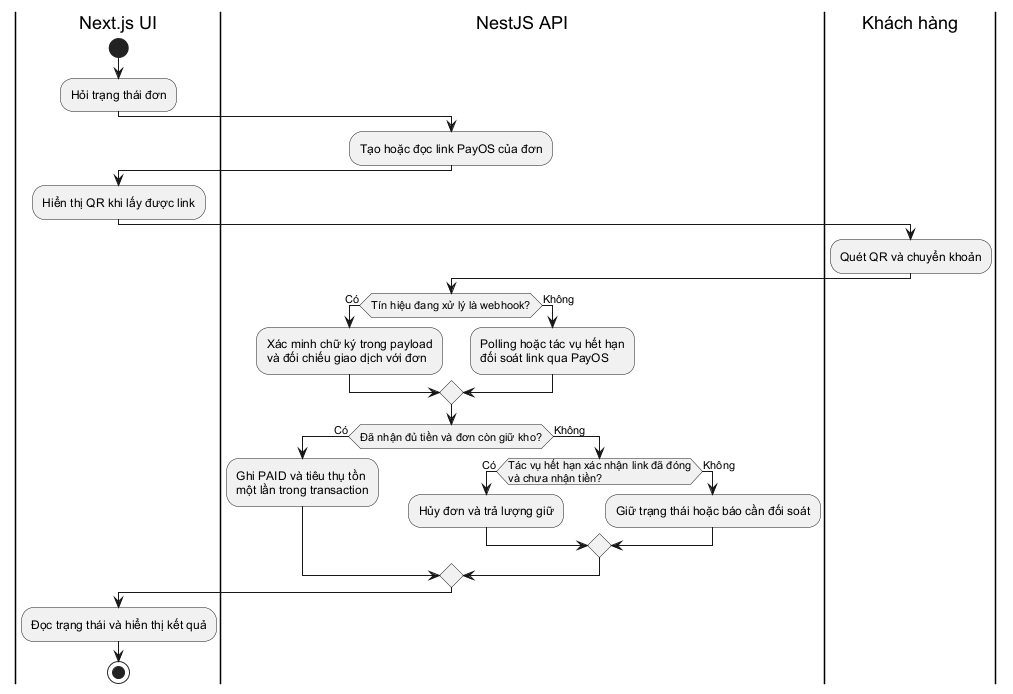
\includegraphics[width=\linewidth,height=0.70\textheight,keepaspectratio]{../../diagrams/activity-payos-webhook.png}\\[0.5em]
{\small\itshape Hình 2.1d. Xác minh giao dịch VietQR và xử lý hết hạn}
\end{center}
